\section{Synthetic Tabular Data generation with \modelname}
Figure~\ref{fig:framework} gives an overview of \modelname.
In Section~\ref{sec:definition}, we first formally define the tabular data generation task. Then, we introduce the design details of \modelname's autoencoding and diffusion process in Section~\ref{sec:vae} and~\ref{sec:diffusion}. We summarize the training and sampling algorithms in Appendix~\ref{appendix:algorithm}. 
\begin{figure}[t]
    \centering
    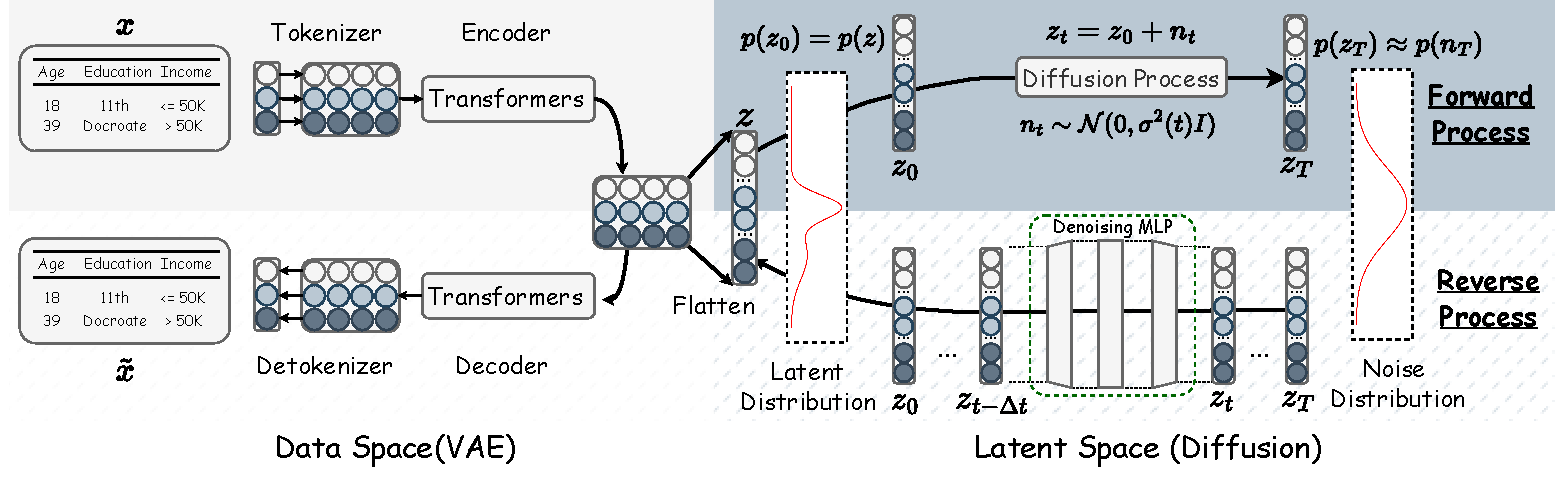
\includegraphics[width = 1.0\linewidth]{Fig/tabsyn_model.pdf} 
    \caption{An overview of the proposed \modelname. Each row data $x$ is mapped to latent space $z$ via a column-wise tokenizer and an encoder. A diffusion process $z_0 \rightarrow z_T$ is applied in the latent space. Synthesis $z_T \rightarrow z_0$ starts from the base distribution $p(z_T)$ and generates samples $z_0$ in latent space through a reverse process. These samples are then mapped from latent $z$ to data space $\tilde{x}$ using a decoder and a detokenizer. }
    \label{fig:framework}
    \vspace{-16pt}
\end{figure}
\subsection{Problem Definition of Tabular Data Generation}\label{sec:definition}
Let $M_{\num}$ and $M_{\cat}$ be the number of numerical columns and categorical columns, respectively. Each row is represented as a vector of numerical features and categorical features $\vx = [\vx^{\num}, \vx^{\cat}]$, where $\vx^{\num} \in \sR^{M_{\num}}$ and $\vx^{\cat} \in \sR^{M_{\cat}} $. Specifically, the $i$-th categorical attribute has $C_i$ finite candidate values, therefore we have $x_{i}^{\cat} \in \{1, \cdots, {C_i} \}, \forall i$.  This paper focuses on the \textbf{unconditional generation} task. With a tabular dataset $\gT = \{\vx\}$, we aim to learn a parameterized generative model $p_{\theta}(\gT)$, with which realistic and diverse synthetic tabular data $\hat{\vx} \in \hat{\gT}$ can be generated.

\subsection{AutoEncoding for Tabular Data}\label{sec:vae}
Tabular data is highly structured of mixed-type column features, with different columns having distinct meanings and being highly dependent on each other. These characteristics make it challenging to design an approximate encoder to model and effectively utilize the rich relationships between columns. Motivated by the successes of Transformers in classification/regression of tabular data~\citep{ft-transformer}, we first learn a unique tokenizer for each column, and then the token(column)-wise representations are fed into a Transformer for capturing the intricate relationships among columns.

\textbf{Feature Tokenizer}. The feature tokenizer converts each column (both numerical and categorical) into a $d$-dimensional vector.  First, we use one-hot encoding to pre-process categorical features, i.e., $ x_{i}^{\cat} \Rightarrow \vx_{i}^{\oh} \in \sR^{1 \times C_i} $. Each record is represented as $\vx = [\vx^{\num}, \vx_{1}^{\oh}, \cdots, \vx_{M_{\cat}}^{\oh}] \in \sR^{M_{\num} + \sum_{i=1}^{M_{\cat}}C_i}$. Then, we apply a linear transformation for numerical columns and create an embedding lookup table for categorical columns, where each category is assigned a learnable $d$-dimensional vector, i.e., 
\begin{equation}\label{eqn:tokenizer}
\begin{split} 
    \ve^{\num}_i  = x^{\num}_i\cdot \vw^{\num}_i + \vb_i^{\num}, \; \;  \ve^{\cat}_i  =  {\vx}^{\oh}_i \cdot \mW^{\cat}_i + \vb^{\cat}_i,
\end{split}
\end{equation}
where $\vw^{\num}_i, \vb^{\num}_i, \vb^{\cat}_i \in \sR^{1 \times d}$, $\mW^{\cat}_i \in \sR^{C_i \times d}$ are learnable parameters of the tokenizer, $\ve^{\num}_i, \ve^{\cat}_i\in \sR^{1 \times d}$.
Now, each record is expressed as the stack of the embeddings of all columns
\begin{equation}
    \mE = [\ve^{\num}_{1}, \cdots, \ve^{\num}_{M_{\num}}, \ve^{\cat}_{1}, \cdots, \ve^{\cat}_{M_{\cat}}] \in \sR^{M \times d}.
\end{equation}

\textbf{Transformer Encoding and Decoding}. As with typical VAEs, we use the encoder to obtain the mean and log variance of the latent variable. Then, we acquire the latent embeddings with the reparameterization tricks. The latent embeddings are then passed through the decoder to obtain the reconstructed token matrix $\hat{\mE} \in \sR^{M\times d}$. The detailed architectures are in Appendix~\ref{appendix:architecture}.

\textbf{Detokenizer}. Finally, we apply a detokenizer to the recovered token representation of each column to reconstruct the column values. The design of the detokenizer is symmetrical to that of the tokenizer:
\begin{equation}\label{eqn:detokenizer}
\begin{split}
    & \hat{x}^{\num}_i = {{\hat{\ve}}^{\num}_i} \cdot \hat{\vw}_i^{\num} + \hat{b}^{\num}_i, \; \; \hat{\vx}^{\oh}_i = {\rm Softmax} ({\hat{\ve}^{\cat}_i} \cdot \hat{\mW}_i^{\cat} + \hat{\vb}^{\cat}_i ), \\
    & \hat{\vx}   = [{\hat{x}}^{\num}_{1} , \cdots, {\hat{x}}^{\num}_{M_{\num}}, {\hat{\vx}}^{\oh}_{1} , \cdots, {\hat{\vx}}^{\oh}_{M_{\cat}}],
\end{split}
\end{equation}
where $\hat{\vw}^{\num}_i \in \sR^{d \times 1}, \hat{b}^{\num}_i \in \sR^{1 \times 1}$, $\mW^{\cat}_i \in \sR^{d \times C_i}, \hat{\vb}^{\cat}_i \in \sR^{1 \times C_i}$ are detokenizer's parameters.

\paragraph{Training with adaptive weight coefficient.} The VAE model is usually learned with the classical ELBO loss function, but here we use $\beta$-VAE~\citep{beta-vae}, where a coefficient $\beta$ balances the importance of the reconstruction loss and KL-divergence loss
\begin{equation}\label{eqn:beta-vae}
\begin{split}
    \gL = \ell_{\rm {recon}} (\vx, \hat{\vx}) + \beta \ell_{\rm kl}.
\end{split}
\end{equation}
$\ell_{\rm recon}$ is the reconstruction loss between the input data and the reconstructed one, and $\ell_{\rm kl}$ is the KL divergence loss that regularizes the mean and variance of the latent space. In the vanilla VAE model, $\beta$ is set to be $1$ because the two loss terms are equally important to generate high-quality synthetic data from Gaussian noises. However, in our model, $\beta$ is expected to be smaller, as we do not require the distribution of the embeddings to precisely follow a standard Gaussian distribution because we have an additional diffusion model. Therefore, we propose to adaptively schedule the scale of $\beta$  in the training process, encouraging the model to achieve lower reconstruction error while maintaining an appropriate embedding shape.

With an initial (maximum) $\beta = \beta_{\rm max}$, we monitor the epoch-wise reconstruction loss $\ell_{\rm recon}$. When $\ell_{\rm recon} $ fails to decrease for a predefined number of epochs (which indicates that the KL-divergence dominates the overall loss), the weight is scheduled by $\beta = \lambda \beta, \lambda < 1$. This process continues until $\beta$ approaches a predefined minimum value $\beta_{\min}$. This strategy is simple yet very effective, and we empirically justify the effectiveness of the design in Section~\ref{sec:exp}.

\subsection{Score-based Generative Modeling in the Latent Space}\label{sec:diffusion}
\paragraph{Training and sampling via denoising.}
After the VAE model is well-learned, we extract the latent embeddings through the encoder and flatten the encoder's output as $\vz = {\rm Flatten}({\rm Encoder} (\vx)) \in \sR^{1 \times Md}$ such that the embedding of a record is a vector rather than a matrix. To learn the underlying distribution of embeddings $p(\vz)$, we consider the following forward diffusion process and reverse sampling process~\citep{vp, edm}:
\begin{align}
    \vz_t & =  \vz_0 + \sigma(t) \bm{\varepsilon}, \; \bm{\varepsilon} \sim \gN(\bm{0}, \mI), & (\text{Forward Process})  \label{eqn:forward}\\
    {\rm d}\vz_t & =  -2\dot{\sigma}(t) \sigma(t) \nabla_{\vz_t} \log p(\vz_t) {\rm d}t + \sqrt{2\dot{\sigma}(t) \sigma(t)} {\rm d} \bm{\omega}_t,  & (\text{Reverse Process}) \label{eqn:reverse}
\end{align}
where $\vz_0 = \vz$ is the initial embedding from the encoder, $\vz_t$ is the diffused embedding at time $t$, and $\sigma(t)$ is the noise level. In the reverse process, $\nabla_{\vz_t} \log p_t(\vz_t)$ is the score function of $\vz_t$, and $\bm{\omega}_t$ is the standard Wiener process. The training of the diffusion model is achieved via denoising score matching~\citep{edm}:
\begin{equation}\label{eqn:denosing}
    \mathcal{L} = \sE_{\vz_0 \sim p(\vz_0)} \sE_{t \sim p(t)} \sE_{\bm{\varepsilon}\sim \gN(\bm{0}, \mI)} \Vert \bm{\epsilon}_{\theta}(\vz_t, t) - \bm{\varepsilon}\Vert_2^2, \;~\text{where}~ \vz_t = \vz_0 + \sigma(t)\bm{\varepsilon},
\end{equation}
where $\bm{\epsilon}_{\theta}$ is a neural network (named denoising function) to approximate the Gaussian noise using the perturbed data $\vx_t$ and the time $t$. Then $\nabla_{\vz_t} \log p(\vz_t) = - {\bm{\epsilon}_{\theta} (\vz_t, t)}/{\sigma(t)}$. After the model is trained, synthetic data can be obtained via the reverse process in Eq.~\ref{eqn:reverse}. The detailed algorithm description of \modelname is provided in Appendix~\ref{appendix:algorithm}. Detailed derivations are in Appendix~\ref{appendix:diffusion}.

\paragraph{Schedule of noise level $\sigma(t)$.} The noise level $\sigma(t)$ defines the scale of noises for perturbing the data at different time steps and significantly affects the final Differential Equation solution trajectories~\citep{vp, edm}. Following the recommendations in~\citet{edm}, we set the noise level $\sigma(t) = t$ that is linear w.r.t. the time. We show in Proposition~\ref{prop:linear} that the linear noise level schedule leads to the smallest approximation errors in the reverse process:
\begin{proposition}\label{prop:linear}
    Consider the reverse diffusion process in Equation~(\ref{eqn:reverse}) from $\vz_{t_b}$ to $\vz_{t_a} (t_b > t_a)$, the numerical solution $\hat{\vz}_{t_a}$ has the smallest approximation error to $\vz_{t_a}$ when $\sigma(t) = t$.
\end{proposition}
See proof in Appendix~\ref{appendix:proof}. A natural corollary of Proposition~\ref{prop:linear} is that a small approximation error allows us to increase the interval between two timesteps, thereby reducing the overall number of sampling steps and accelerating the sampling. In Section~\ref{sec:exp}, we demonstrate that with this design, \modelname can generate synthetic tabular data of high quality within less than $20$ NFEs (number of function evaluations), which is much smaller than other tabular-data synthesis methods based on diffusion~\citep{stasy, tabddpm}.
